% !TeX root = ../../main.tex
\subsection{証明}

証明の流れと型を身につけてもらいたい. 学校の型と異なるかとは思うが, ここでは私がオススメする型を紹介する.
特にこだわりがない場合は, この型を是非使ってもらいたい.

ここで使用する流れや型は2年次で学習する「合同な図形」の証明においても, 3年次で学習する「相似な図形」の証明においても使用できる汎用的なものである.

\begin{theorembox}{\textbf{証明の流れ}}
    \label{thm:証明の流れ}
    証明の流れは以下のようになる.

    \begin{enumerate}
        \item \fitblankbf[証明したい図形]{} を確認し, 一方を \fitblankbf[赤い三角形]{} で, もう一方を \fitblankbf[青い三角形]{} で囲む.
        \item 赤い三角形と青い三角形を \fitblankbf[抜き出し]{} $^{*}$, \fitblankbf[仮定]{} や \fitblankbf[条件]{} を描き込む.
        \item (2)で抜き出した図形をもとに \fitblankbf[合同条件]{} を確定させる. $^{**}$
    \end{enumerate}
\end{theorembox}

Theorem \ref{thm:証明の流れ} で証明の下準備は完了! 証明は書き始める前に終えてなければならない.
したがって, Theorem \ref{thm:証明の流れ} を使って証明の型にはめていくことになる.

\begin{theorembox}{\textbf{証明の型}}
    \label{thm:証明の型}
    証明の型は以下のようになる. ここでは \textcolor{red}{\underline{$\triangle ABC$}} と \textcolor{blue}{\underline{$\triangle DEF$}} が合同であることを証明する.
\vspace{-1.5em}
    \begin{proof}
        \setlength{\baselineskip}{1.5\baselineskip}
        \mbox{}\\
        \textcolor{red}{\fitblankbf[\triangle ABC]{} } と \textcolor{blue}{\fitblankbf[\triangle DEF]{} } において

        \vspace{0.3em}
        \textcolor{black}{\uwave{\hspace{2em}根拠①\hspace{3em}}} より,

        \vspace{0.3em}
        \makebox[\linewidth][s]{\textcolor{red}{\fitblankbf[AB]{} } = \textcolor{blue}{\fitblankbf[DE]{} } \hfill ・・・①}

        \vspace{0.3em}
        \textcolor{black}{\uwave{\hspace{2em}根拠②\hspace{3em}}} ので,

        \vspace{0.3em}
        \makebox[\linewidth][s]{\textcolor{red}{\fitblankbf[\angle BAC]{} } = \textcolor{blue}{\fitblankbf[\angle EDF]{} } \hfill ・・・②}

        \vspace{0.3em}
        \textcolor{black}{\uwave{\hspace{2em}根拠③\hspace{3em}}} ので,

        \vspace{0.3em}
        \makebox[\linewidth][s]{\textcolor{red}{\fitblankbf[CA]{} } = \textcolor{blue}{\fitblankbf[FD]{} } \hfill ・・・③}

        \vspace{0.3em}
        ①, ②, ③より, \textcolor{black}{\fitblankbf[合同条件]{} } ので,

        \vspace{0.3em}
        \textcolor{red}{\fitblankbf[\triangle ABC]{} } $\equiv$ \textcolor{blue}{\fitblankbf[\triangle DEF]{} }
    \end{proof}
\end{theorembox}
\vspace{-2em}
\vfill
\noindent\rule{\textwidth}{0.4pt}

\vspace{0.2em}
\noindent
$^{*}$ 図形を抜き出す際には \textbf{形は気にせず} 抜き出してもらって構わない. しかし, 2つの三角形とも \textbf{同じ形} で
\textbf{対応する頂点} で抜き出すこと.

$^{**}$ 合同条件の確定には \textbf{結論} を使ってはならない.

\newpage

% 例題4.1
\begin{example}
    \noindent
    \begin{minipage}[t]{0.5\textwidth}
        \vspace{0pt}
        右の図において、 $AB = DC$、 $AB \rotatebox[origin=c]{-25}{$\parallel$} DC$ ならば
        $\triangle ABC \equiv \triangle CDA$ であることを証明しなさい。
    \end{minipage}\hfill
    \begin{minipage}[t]{0.5\textwidth}
        \vspace{0pt}
        \centering
        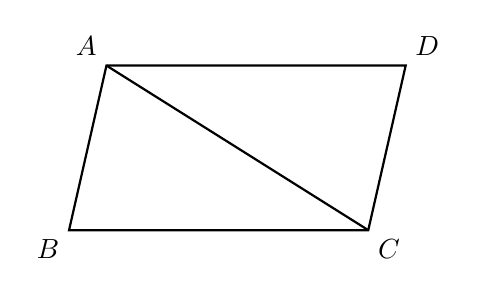
\begin{tikzpicture}[scale=0.95]
            \coordinate (A) at (0,2.2);
            \coordinate (B) at (-0.5,0);
            \coordinate (C) at (3.5,0);
            \coordinate (D) at (4,2.2);
            \draw[thick] (A) -- (B) -- (C) -- (D) -- cycle;
            \draw[thick] (A) -- (C);
            \fill (A) node[above left] {$A$};
            \fill (B) node[below left] {$B$};
            \fill (C) node[below right] {$C$};
            \fill (D) node[above right] {$D$};
        \end{tikzpicture}
    \end{minipage}
\end{example}

\begin{proof}\mbox{}\\
    \begin{hiddenanswer}
        $\triangle ABC$ と $\triangle CDA$ において

        \vspace{0.5em}
        仮定より,

        \vspace{0.3em}
        \makebox[\linewidth][s]{$AB = CD$ \hfill ・・・①}

        \vspace{0.3em}
        $AB \rotatebox[origin=c]{-25}{$\parallel$} DC$ より, 平行線の錯角は等しいから,

        \vspace{0.3em}
        \makebox[\linewidth][s]{$\angle BAC = \angle DCA$ \hfill ・・・②}

        \vspace{0.3em}
        共通な辺であるから,

        \vspace{0.3em}
        \makebox[\linewidth][s]{$AC = CA$ \hfill ・・・③}

        \vspace{0.3em}
        ①, ②, ③より, 2組の辺とその間の角がそれぞれ等しいので,

        \vspace{0.3em}
        $\triangle ABC \equiv \triangle CDA$
    \end{hiddenanswer}
\end{proof}
\newpage

% 例題4.2
\begin{example}
    \noindent
    \begin{minipage}[t]{0.5\textwidth}
        \vspace{0pt}
        右の図において、 $AB = DC$、 $\angle ABC = \angle DCB$ ならば
        $\angle BAC = \angle CDB$ であることを証明しなさい。
    \end{minipage}\hfill
    \begin{minipage}[t]{0.5\textwidth}
        \vspace{0pt}
        \centering
        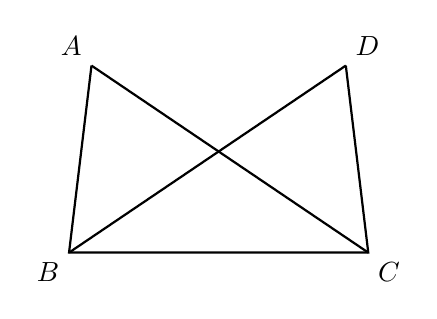
\begin{tikzpicture}[scale=0.95]
            \usetikzlibrary{angles,calc}
            \coordinate (B) at (-0.3,0);
            \coordinate (C) at (3.7,0);
            \coordinate (A) at (0,2.5);
            \coordinate (D) at (3.4,2.5);
            \draw[thick] (A) -- (B) -- (C) -- (D);
            \draw[thick] (A) -- (C);
            \draw[thick] (D) -- (B);
            \fill (A) node[above left] {$A$};
            \fill (B) node[below left] {$B$};
            \fill (C) node[below right] {$C$};
            \fill (D) node[above right] {$D$};
        \end{tikzpicture}
    \end{minipage}
\end{example}
\vspace{-2em}

\begin{proof}\mbox{}\\
    \begin{hiddenanswer}
        $\triangle ABC$ と $\triangle DCB$ において

        \vspace{0.5em}
        仮定より,

        \vspace{0.3em}
        \makebox[\linewidth][s]{$AB = DC$ \hfill ・・・①}

        \vspace{0.3em}
        \makebox[\linewidth][s]{$\angle ABC = \angle DCB$ \hfill ・・・②}

        \vspace{0.3em}
        共通な辺であるから,

        \vspace{0.3em}
        \makebox[\linewidth][s]{$BC = CB$ \hfill ・・・③}

        \vspace{0.3em}
        ①, ②, ③より, 2組の辺とその間の角がそれぞれ等しいので,

        \vspace{0.3em}
        $\triangle ABC \equiv \triangle DCB$

        \vspace{0.3em}
        合同な図形では対応する角の大きさは等しいから,

        \vspace{0.3em}
        $\angle BAC = \angle CDB$
    \end{hiddenanswer}
\end{proof}
